\chapter{Metodo Perona-Malik}

Il metodo Perona-Malik, come anticipato, si basa sull'equazione del calore. L'idea è quella di applicare tale equazione lontano dai bordi dell'immagine e mantenere invece inalterati quest'ultimi.
Questo metodo risulta particolarmente efficace per risolvere problemi di disturbo come ad esempio un rumore del tipo salt and pepper, cioè con dei pixel bianchi o neri sparsi per la foto.\\
\vspace{1em}
\`E bene capire da un punto di vista prettamente matematico cosa vuol dire che il metodo si basa sull'equazione del calore, che ricordiamo essere:\\
\begin{equation} 
\begin{cases}
\frac{\partial u}{\partial t}(t,x)-\Delta u(t,x) = 0 \ x \in \mathbb R^2, t\ge 0 \ .\\ 
u(0,x) = u_0(x)\ . \\
\end{cases}
\end{equation}
Il laplaciano è la divergenza del gradiente, ed è qui che viene operata la modifica.
Come detto: $\Delta(u)=div(\nabla(u))$, volendo operare un controllo si introdurrà un coefficente k $div(k\nabla(u))$, nel caso esso sia uno scalare costante, avremo $k\Delta(u)=div(\nabla(u))$ ed è il caso implementato nelle pagine precendenti. Il metodo Perona-Malik invece prevede l'impego di un coefficiente k non costante, ma che cambi a seconda del pixel su cui si opera. In questo senso, questo filtro viene detto di diffusione anisotropa. Il termine anisotropo indica come la diffusione sia diversa nelle varie direzioni, capiamo quindi come questa notazione, per quanto esplicativa sia in verità un abuso di notazione siccome la diffusione non avviene in direzioni diverse ma semplicemente con intensità diverse. Esistono tuttavia dei metodi metodi di diffusione anisotropa, in tal caso k sarà un tensore variabile.\\
Ritornando al metodo in esame, il problema affrontato diventa\\
\begin{equation} 
\begin{cases}
\frac{\partial u}{\partial t}(t,x)-div(c(|\nabla(u)|^2)\nabla(u)) = 0 \ x \in \mathbb R^2, t\ge 0 \ .\\ 
\frac{\partial u}{\partial N}=0 \ x \in \mathbb R^2, t\ge 0 \ .\\ 
u(0,x) = u_0(x)\ . \\
\end{cases}
\end{equation}
Servirà dunque esplicitare e discretizzare questo problema, per fare ciò saranno impiegati, oltre ai metodi già visti, altri accorgimenti.\\

\newpage
\section{Soluzione discreta della PDE}
Preso un punto si può operare la derivata nelle 4 direzioni, e saranno numericamente simili a due a due. In particolare in direzioni opposte avranno segni invertiti, possono quindi essere utilizzate per il calcolo del gradiente.
Visto che la divergenza è la somma delle derivate parziali, si può pensare di calcolare anche il coefficiente in base alla direzione, così, essendo uno scalare, lo si può portare fuori e fare semplicemente la somma dei prodotti coefficente-derivata.\\
La soluzione discreta della PDE sarà quindi:\\
$$
u = u + dt*(k_N\nabla_N + k_S\nabla_S + k_W\nabla_W + k_E\nabla_E );
$$
 

\section{Maschere di convoluzione}
Per implementare il filtro di diffusione anisotropica detto "Perona-Malik", ci serviremo dunque di alcune \textbf{maschere}.\\
Un filtro è una funzione $F:\mathbb R^2\to\mathbb R$, in quanto tale avrà un nucleo $\operatorname{Ker}(F):=\{v \in \mathbb R^2: Av=0\}$ che sarà un polinomio a due incognite. Date in input a tale polinomio delle coordinate, questo restituirà un valore numerico, chiameremo tale coefficiente \textbf{peso}. Compiliamo quindi una maschera con i pesi calcolati in tal modo per ogni posizione ottenendo una cosa del tipo:

\begin{figure}[]
    \centering
    \begin{tabular}{|p{1.6cm}|p{1.6cm}|p{1.6cm}|}
        \hline
        \makebox[1.6cm][c]{
        \rule[-8mm]{0cm}{1.6cm}
        $a_1$} & 
        \makebox[1.6cm][c]{
        $a_2$} & 
        \makebox[1.6cm][c]{
        $a_3$} \\
        \hline
        \makebox[1.6cm][c]{
        \rule[-8mm]{0cm}{1.6cm}
        $a_4$} & 
        \makebox[1.6cm][c]{
        $a_5$} & 
        \makebox[1.6cm][c]{
        $a_6$} \\
        \hline
        \makebox[1.6cm][c]{
        \rule[-8mm]{0cm}{1.6cm}
        $a_7$} & 
        \makebox[1.6cm][c]{
        $a_8$} & 
        \makebox[1.6cm][c]{
        $a_9$} \\
        \hline
    \end{tabular}
    \caption{Esempio di maschera di convoluzione 3x3}
    \label{fig:my_label}
\end{figure}
Le dimensioni della maschera possono variare a discrezione del programmatore ma, solitamente si utilizzano maschere dimensioni piccole e dispari. Dispari perchè è importante individuare il centro della maschera. Piccole perchè l'utilizzo delle maschere porta degli effetti bordo che è bene limitare. queste motivazioni verranno meglio spiegate a breve.\\
\vspace{1em}
Come detto nelle nozioni introduttive, applicare un filtro vuol dire operare una convoluzione tra due funzioni: l'immagine ed il filtro stesso.\\
Le maschere sono un utile strumento proprio per il calcolo delle convoluzioni, motivo per cui sono solitamente dette \textbf{maschere di convoluzione}. Per operare una convoluzione,detti $u:\mathbb R^2\to\mathbb R$ l'immagine e $F:\mathbb R^2\to\mathbb R$ il filtro, per definizione, $\forall p_{i,j}\in dom(u)$ si prende un intorno I(p), le cui dimensioni dipendono da quelle della maschera scelta per F. Successivamente si sommano i prodotti tra i valori di u e quelli di F, cioè i pesi della maschera, per ottenere in fine l'immagine filtrata.\\
\vspace{1em}
In pratica, si scorre la maschera sui vari pixel dell'immagine\\
\begin{figure}[h!]
    \centering
    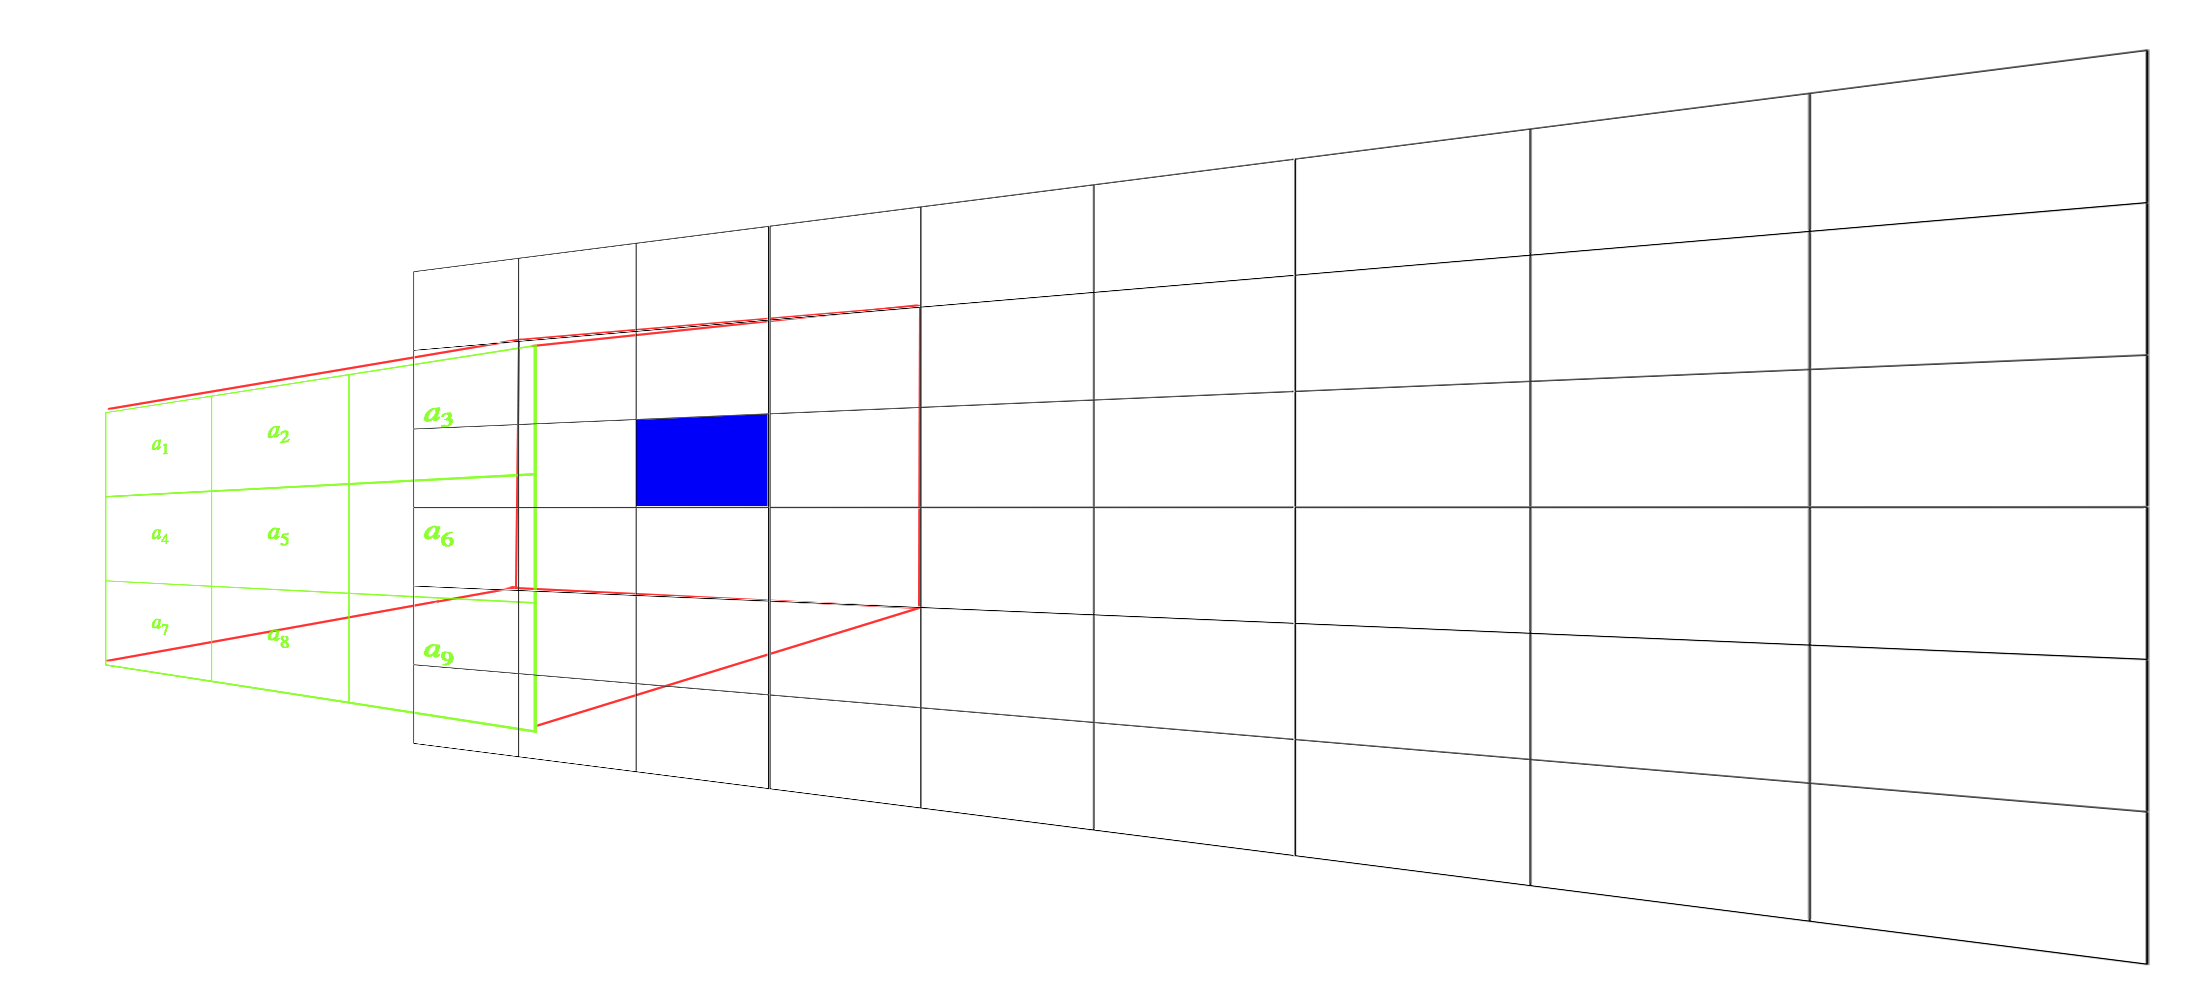
\includegraphics[scale=0.15]{Pictures/illustrazione convoluzione.png}
    \caption{Griglia dell'immagine in nero, maschera in verde, pixel in esame in blu}
    \label{fig:my_label}
\end{figure}
Per ogni pixel ne viene ricalcolato il valore come segue
\begin{figure}
    \centering
    %\begin{tabular}{|c|c|c|}
    \begin{tabular}{|p{1.6cm}|p{1.6cm}|p{1.6cm}|}
        \hline
        \makebox[1.6cm][c]{
        \rule[-8mm]{0cm}{1.6cm}
        $p_{i-1,j+1}$} & 
        \makebox[1.6cm][c]{
        $p_{i,j+1}$} & 
        \makebox[1.6cm][c]{
        $p_{i+1,j+1}$} \\
        \hline
        \makebox[1.6cm][c]{
        \rule[-8mm]{0cm}{1.6cm}
        $p_{i-1,j}$} & 
        \makebox[1.6cm][c]{
        $p_{i,j}$} & 
        \makebox[1.6cm][c]{
        $p_{i+1,j}$} \\
        \hline
        \makebox[1.6cm][c]{
        \rule[-8mm]{0cm}{1.6cm}
        $p_{i-1,j-1}$} & 
        \makebox[1.6cm][c]{
        $p_{i,j-1}$} & 
        \makebox[1.6cm][c]{
        $p_{i+1,j-1}$} \\
        \hline
    \end{tabular}
    \hspace{1em}
    \huge{*}
    \normalsize
    \hspace{1em}
    \begin{tabular}{|p{1.6cm}|p{1.6cm}|p{1.6cm}|}
        \hline
        \makebox[1.6cm][c]{
        \rule[-8mm]{0cm}{1.6cm}
        $a_1$} & 
        \makebox[1.6cm][c]{
        $a_2$} & 
        \makebox[1.6cm][c]{
        $a_3$} \\
        \hline
        \makebox[1.6cm][c]{
        \rule[-8mm]{0cm}{1.6cm}
        $a_4$} & 
        \makebox[1.6cm][c]{
        $a_5$} & 
        \makebox[1.6cm][c]{
        $a_6$} \\
        \hline
        \makebox[1.6cm][c]{
        \rule[-8mm]{0cm}{1.6cm}
        $a_7$} & 
        \makebox[1.6cm][c]{
        $a_8$} & 
        \makebox[1.6cm][c]{
        $a_9$} \\
        \hline
    \end{tabular}
    \small{
    $$
    u(p_{i,j})*a=a_1p_{i-1,j+1} + a_2p_{i,j+1} + a_3p_{i+1,j+1} + a_4p_{i-1,j} + a_5p_{i,j} + a_6p_{i+1,j} + a_7p_{i-1,j-1} + a_8p_{i,j-1} + a_9p_{i+1,j-1}.
    $$
    }\\
\caption{Intorno di un punto, maschera di convoluzione e soluzione analitica}
\label{fig:my_label}
\end{figure}

\vspace{-1em}

Ma allora una convoluzione con $a=$
    \begin{tabular}{|p{0.4cm}|p{0.4cm}|p{0.4cm}|}
        \hline
        \makebox[0.4cm][c]{
        \rule[-2mm]{0cm}{0.6cm}
        $0$} & 
        \makebox[0.4cm][c]{
        $1$} & 
        \makebox[0.4cm][c]{
        $0$} \\
        \hline
        \makebox[0.4cm][c]{
        \rule[-2mm]{0cm}{0.6cm}
        $0$} & 
        \makebox[0.4cm][c]{
        $-1$} & 
        \makebox[0.4cm][c]{
        $0$} \\
        \hline
        \makebox[0.4cm][c]{
        \rule[-2mm]{0cm}{0.6cm}
        $0$} & 
        \makebox[0.4cm][c]{
        $0$} & 
        \makebox[0.4cm][c]{
        $0$} \\
        \hline
    \end{tabular}
\vspace{0.5em}
vuol dire fare la derivata prima approssimata alle differenze finite lungo y, in particolare verso l'alto, infatti facendo il conto di cui sopra si ottiene $u(p_{i,j})*a=p_{i,j+1}-p_{i,j}$ che è esattamente quanto trovato analizzando il metodo alle differenze finite
si può operare analogamente in tutte e 4 le direzioni.\\
\vspace{1em}
Per facilitare la successiva implementazione del filtro, si è scritta una funzione MATLAB che operi in tal senso.

\begin{lstlisting}[language=MATLAB]
function B=convoluzione(A,k);

[r c] = size(A);            %Memorizzo le dimensioni dell'immagine
[m n] = size(k);            %Memorizzo le dimensioni della maschera
h = rot90(k, 2);

%Definisco una cornice per gestire gli effetti di bordo
center = floor((size(h)+1)/2);                  
left = center(2) - 1;
right = n - center(2);
top = center(1) - 1;
bottom = m - center(1);

%Preparo un "piano di lavoro"
Rep = zeros(r + top + bottom, c + left + right);
for x = 1 + top : r + top
    for y = 1 + left : c + left
        Rep(x,y) = A(x - top, y - left);
    end
end

%Opero la convoluzione
B = zeros(r , c);
for x = 1 : r
    for y = 1 : c
        for i = 1 : m
            for j = 1 : n
                q = x - 1;
                w = y -1;
                B(x, y) = B(x, y) + (Rep(i + q, j + w) * h(i, j));
            end
        end
    end
end

\end{lstlisting}
Notare che \texttt{Rep} ha dimensioni maggiori rispetto all'immagine questo perchè dobbiamo gestire anche i pixel sui bordi del riquadro dell'immagine. Volendo fare un esempio, si consideri il pixel in posizione (1,1), ossia l'angolo in alto a sinistra, allora i coeff $a_1$, $a_2$, $a_3$, $a_4$ e $a_7$, non avranno nessun corrispettivo da moltiplicare, costruiamo quindi una cornice nera (cioè pixel di valore nullo) per ovviare a questo problema. Ovviamente se la maschera è grande, questo porterà a dei visibili errori di bordo, il che è esattamente il motivo per cui si usano solitamente maschere di dimensioni molto piccole.

\newpage 
\section{Problema dei "bordi" d'interferenza}
%\subsection{Considerazioni sui bordi}
%\subsection{Miglioramento dei bordi}
Come evidenziato con l'ultima immagine di prova nella sezione dedicata al rilevamento dei bordi, anche gli elementi di disturbo ne hanno e vengono quindi rilevati. Questo è un problema perchè il metodo Perona-Malik tenderà a preservarli.\\
Per ovviare a questo problema operiamo su di una copia dell'immagine una diffusione come quella operata dall'equazione del calore vista in precedenza, così facendo, in questa copia, i bordi dell'immagine risulteranno roviati, ma non scomparsi! Gli elementi di disturbo saranno invece eliminati.\\
Moltiplicando i due gradienti così trovati si può osservare che: in corrispondenza degli elementi di disturbo il secondo gradiente sarà nullo ed il prodotto sarà dunque anch'esso nullo, vicino ai bordi il secondo gradiente non è nullo, ma il primo sì! Quindi il prodotto sarà ancora nullo, in corrispondenza degli effettivi bordi entrambi i gradienti saranno non nulli e quindi neanche il loro prodotto lo sarà.\\ Questo vuol dire che:\\
\begin{itemize}
    \item gli elementi di disturbo sono stati eliminati
    \item l'effetto distruttivo sui bordi non viene riportato
    \item gli effettivi bordi dell'immagine vengono preservati
\end{itemize}
I bordi sono quindi calcolati in maniera efficiente.\\
\vspace{1em}
\`E doveroso fare ancora una considerazione. Serve applicare ancora una trasformazione ai nostri bordi in modo da risultare ancor più efficienti ai nostri scopi, ossia una funzione di controllo. Cerchiamo una funzione decrescente tale che c(0)=1 (quindi dove non c'è bordo opera l'eq del calore) e $\lim_{s\to\infty}(s)=0$ (quindi tanto più i bordi sono accentuati, tanto più l'eq del calore NON deve operare).
Facciamo questo banalmente perchè considerando semplicemente i bordi, avremmo l'effetto opposto! Infatti dove non ci sono bordi $s=0$ e quindi non ci sarebbe diffusione, dove ci sono bordi molto marcati $s\to\infty$ quindi la diffusione verrebbe adoperata addirittura più del normale!
Non a caso una delle scelte più semplici, anche se non delle più classiche nè efficienti è $\frac{1}{1+s/k}$ dove k è un fattore di controllo.
Scelte decisamente più classiche ed impiegate sono:
\begin{itemize}
    \item $e^{-\frac{s}{k}}$ che preserva maggiromente i bordi ad altro constrasto e meno quelli a basso contrasto
    \item $\frac{1}{\sqrt{1+s/k)}}$ che preserva maggiormente regioni grandi piuttosto che quelle piccole
\end{itemize} 

\newpage
\section{Implementazione}
\begin{lstlisting}[language=MATLAB]

img=imread('nome_file.png');             %Apertura dell'immmagine
img=rgb2gray(img);                     %Trasformazione in bianco e nero


im=uint8(img);
im = imnoise(im,'salt & pepper',0.02);  %Aggiunta del rumore

figure('Name','Original picture');      %Stampa dell'immagine rumorosa
imshow(im);

num_iter=70;                            %numero di iterazioni
delta_t=0.1;                            %costante d'integrazione
kappa=6;                                %coefficiente di controllo del gradiente

sigma=5;                                %varianza della funzione gaussiana

% conversione in double per il calcolo.
im = double(im);

% Condizioni iniziali della PDE.
diff_im = im;


% Maschera di convoluzione
hN = [0 1 0; 0 -1 0; 0 0 0];
hS = [0 0 0; 0 -1 0; 0 1 0];
hE = [0 0 0; 0 -1 1; 0 0 0];
hW = [0 0 0; 1 -1 0; 0 0 0];


for t = 1:num_iter
   
    % Calcolo alle differenze finite nelle 4 direzioni
    nablaN = convoluzione(diff_im,hN);
    nablaS = convoluzione(diff_im,hS);   
    nablaW = convoluzione(diff_im,hW);
    nablaE = convoluzione(diff_im,hE);
    
    diff_blur = imgaussfilt(diff_im,sigma);
    nablaN_blur = convoluzione(diff_blur,hN);
    nablaS_blur = convoluzione(diff_blur,hS);   
    nablaW_blur = convoluzione(diff_blur,hW);
    nablaE_blur = convoluzione(diff_blur,hE);

    cN = exp(-(nablaN_blur/kappa).^2);
    cS = exp(-(nablaS_blur/kappa).^2);
    cW = exp(-(nablaW_blur/kappa).^2);
    cE = exp(-(nablaE_blur/kappa).^2);

    % Soluzione discreta della PDE.
    diff_im = diff_im + delta_t*(cN.*nablaN + cS.*nablaS + cW.*nablaW + cE.*nablaE );
           
    % Stampa di controllo
    fprintf('\rIteration %d\n',t);
end
% Stampa dei risultati
figure('Name','Perona Malik');
imshow(uint8(diff_im));

\end{lstlisting}